\documentclass[conference,onecolumn]{IEEEtran} % or twocolumn
\usepackage{cite}
\usepackage[pdftex]{graphicx}
%\usepackage[cmex10]{amsmath}
%\usepackage{algorithmic}
%\usepackage[tight,footnotesize]{subfigure}
%\usepackage[font=footnotesize]{subfig}
%\usepackage{url}

% correct bad hyphenation here
\hyphenation{op-tical net-works semi-conduc-tor}

\begin{document}
%
% paper title
% can use linebreaks \\ within to get better formatting as desired
\title{CE558 Team2 Project}


% author names and affiliations
% use a multiple column layout for up to three different
% affiliations
\author{
\IEEEauthorblockN{Duckyu Choi}
\IEEEauthorblockA{Dept. Civil and Environmental Engineering\\ KAIST}
}


% make the title area
\maketitle


\begin{abstract}
%\boldmath
The abstract goes here. The abstract goes here. The abstract goes here. The abstract goes here.
The abstract goes here. The abstract goes here. The abstract goes here. The abstract goes here.
The abstract goes here. The abstract goes here. The abstract goes here. The abstract goes here.
\end{abstract}


\section{Introduction}
% no \IEEEPARstart
There are various applications that perform tasks using robots in the current urban environment. In particular, UAV, a platform with excellent access to 3D space, has been used for various missions such as crack inspection of structures, lifesaving in disaster situations, and transportation of goods. However, in most cases, it is often operated based on a prior map, and has not been actually used to obtain new environmental information due to instability in control and low constraints on location information. Accordingly, various studies to obtain environmental information using UAVs in the fields of active slam, exploration, and coverage path planning are actively being conducted. Most of these studies presuppose the designation of the mapping area, such as indoor environments or structures that know the approximate size. This prerequisite is necessary because the termination condition of the control strategy for mapping is unclear, and the ambiguity is originated from the control strategy which prioritizes the free space.

Unlike the NBVP or frontier exploration strategy, which selects the next point in free space next to the unknown area, this paper obtains continuous structure information by designating the next point based on the newly updated map information. This allows the exploration termination condition to be defined not as the ratio of the filled map to the size of the entire given exploration area, but as connectivity of continuous structures to the ground. Moreover, the proposed algorithm can be performed without knowing the approximate size information. In addition, a structure to obtain map information can be expressed as a three-dimensional figure in various and simple forms. In the proposed algorithm, a path suitable for each figure is created, and when two or more figures are recognized in the newly updated map information, a path that prioritizes the currently inspected figure is created by storing the location and shape of the structure in a tree data structure. After that, it creates a path to inspect other recognized shapes. The light-weight clustering technique was used to classify the structure into simple shapes, which considers the characteristics of UAVs that cannot use a high computation module due to low payload. A path suitable for structure mapping was created as a waypoint, and in order to create a smooth path in consideration of the dynamics of the UAV, a continuous minimum jerk path was created in consideration of the start to end point configuration through a motion primitive algorithm.

\subsection{Subsection Heading Here}
Subsection text here. Subsection text here. Subsection text here. Subsection text here.


\subsubsection{Subsubsection Heading Here}
Subsubsection text here. Subsubsection text here. Subsubsection text here. Subsubsection text here.

\begin{figure}[!h]
  \centering
    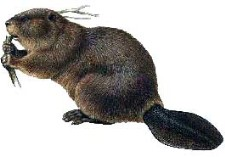
\includegraphics[width=2.5in]{beaver.jpg}
  \caption{Simulation Results}
  \label{figlabel}
\end{figure}

As can be seen in Fig. \ref{figlabel}, example figure can be placed as below.
Subsubsection text here. Subsubsection text here. Subsubsection text here. Subsubsection text here.

\begin{table}[!h]
% increase table row spacing, adjust to taste
\renewcommand{\arraystretch}{1.3}
  \caption{An Example of a Table}
  \label{tablelabel}
  \centering
  \begin{tabular}{|c||c|}
  \hline
  One & Two\\
  \hline
  Three & Four\\
  \hline
  \end{tabular}
\end{table}

As can be seen in \ref{tablelabel}, example table can be placed as below. Subsubsection text here. Subsubsection text here. Subsubsection text here. Subsubsection text here.

\section{Conclusion}
The conclusion goes here. The conclusion goes here. The conclusion goes here. The conclusion goes here This is how to cite a paper \cite{jung2018multi}. Look at references.bib file for more details.

% use section* not to add number in the front
\section*{Acknowledgment}
The authors would like to thank...


% references section
\IEEEtriggeratref{5}
\bibliographystyle{IEEEtran}
\bibliography{references}


% that's all folks
\end{document}


